\chapter{Literature Review}

% Split into two main sections: fields and techniques; mathematical background

% Lit review structure
% ML intro as subset of AI
% NNs
% Note on AI winter
% SVMs
% DL emerges - note on previous aspersions on this
% Image recognition
% Expansion to other domains and architectures
% Acceleration, hype (media coverage, publicity etc, large industrial use Tesla etc)
% Emphasis on loss functions and explanation
% History of Random Projections
% Narrow down to flip probability specifically
% Mention use in logistic regression and bounds on error for linear classification

\section*{Fields and Techniques}

%\begin{SCfigure}
% ZAMBINGO - if possible, redo figure using ggplot
% ZAMBINGO - spelling mistake - should be 'breadth' not 'breath
\begin{wrapfigure}{r}{0.5\textwidth}
    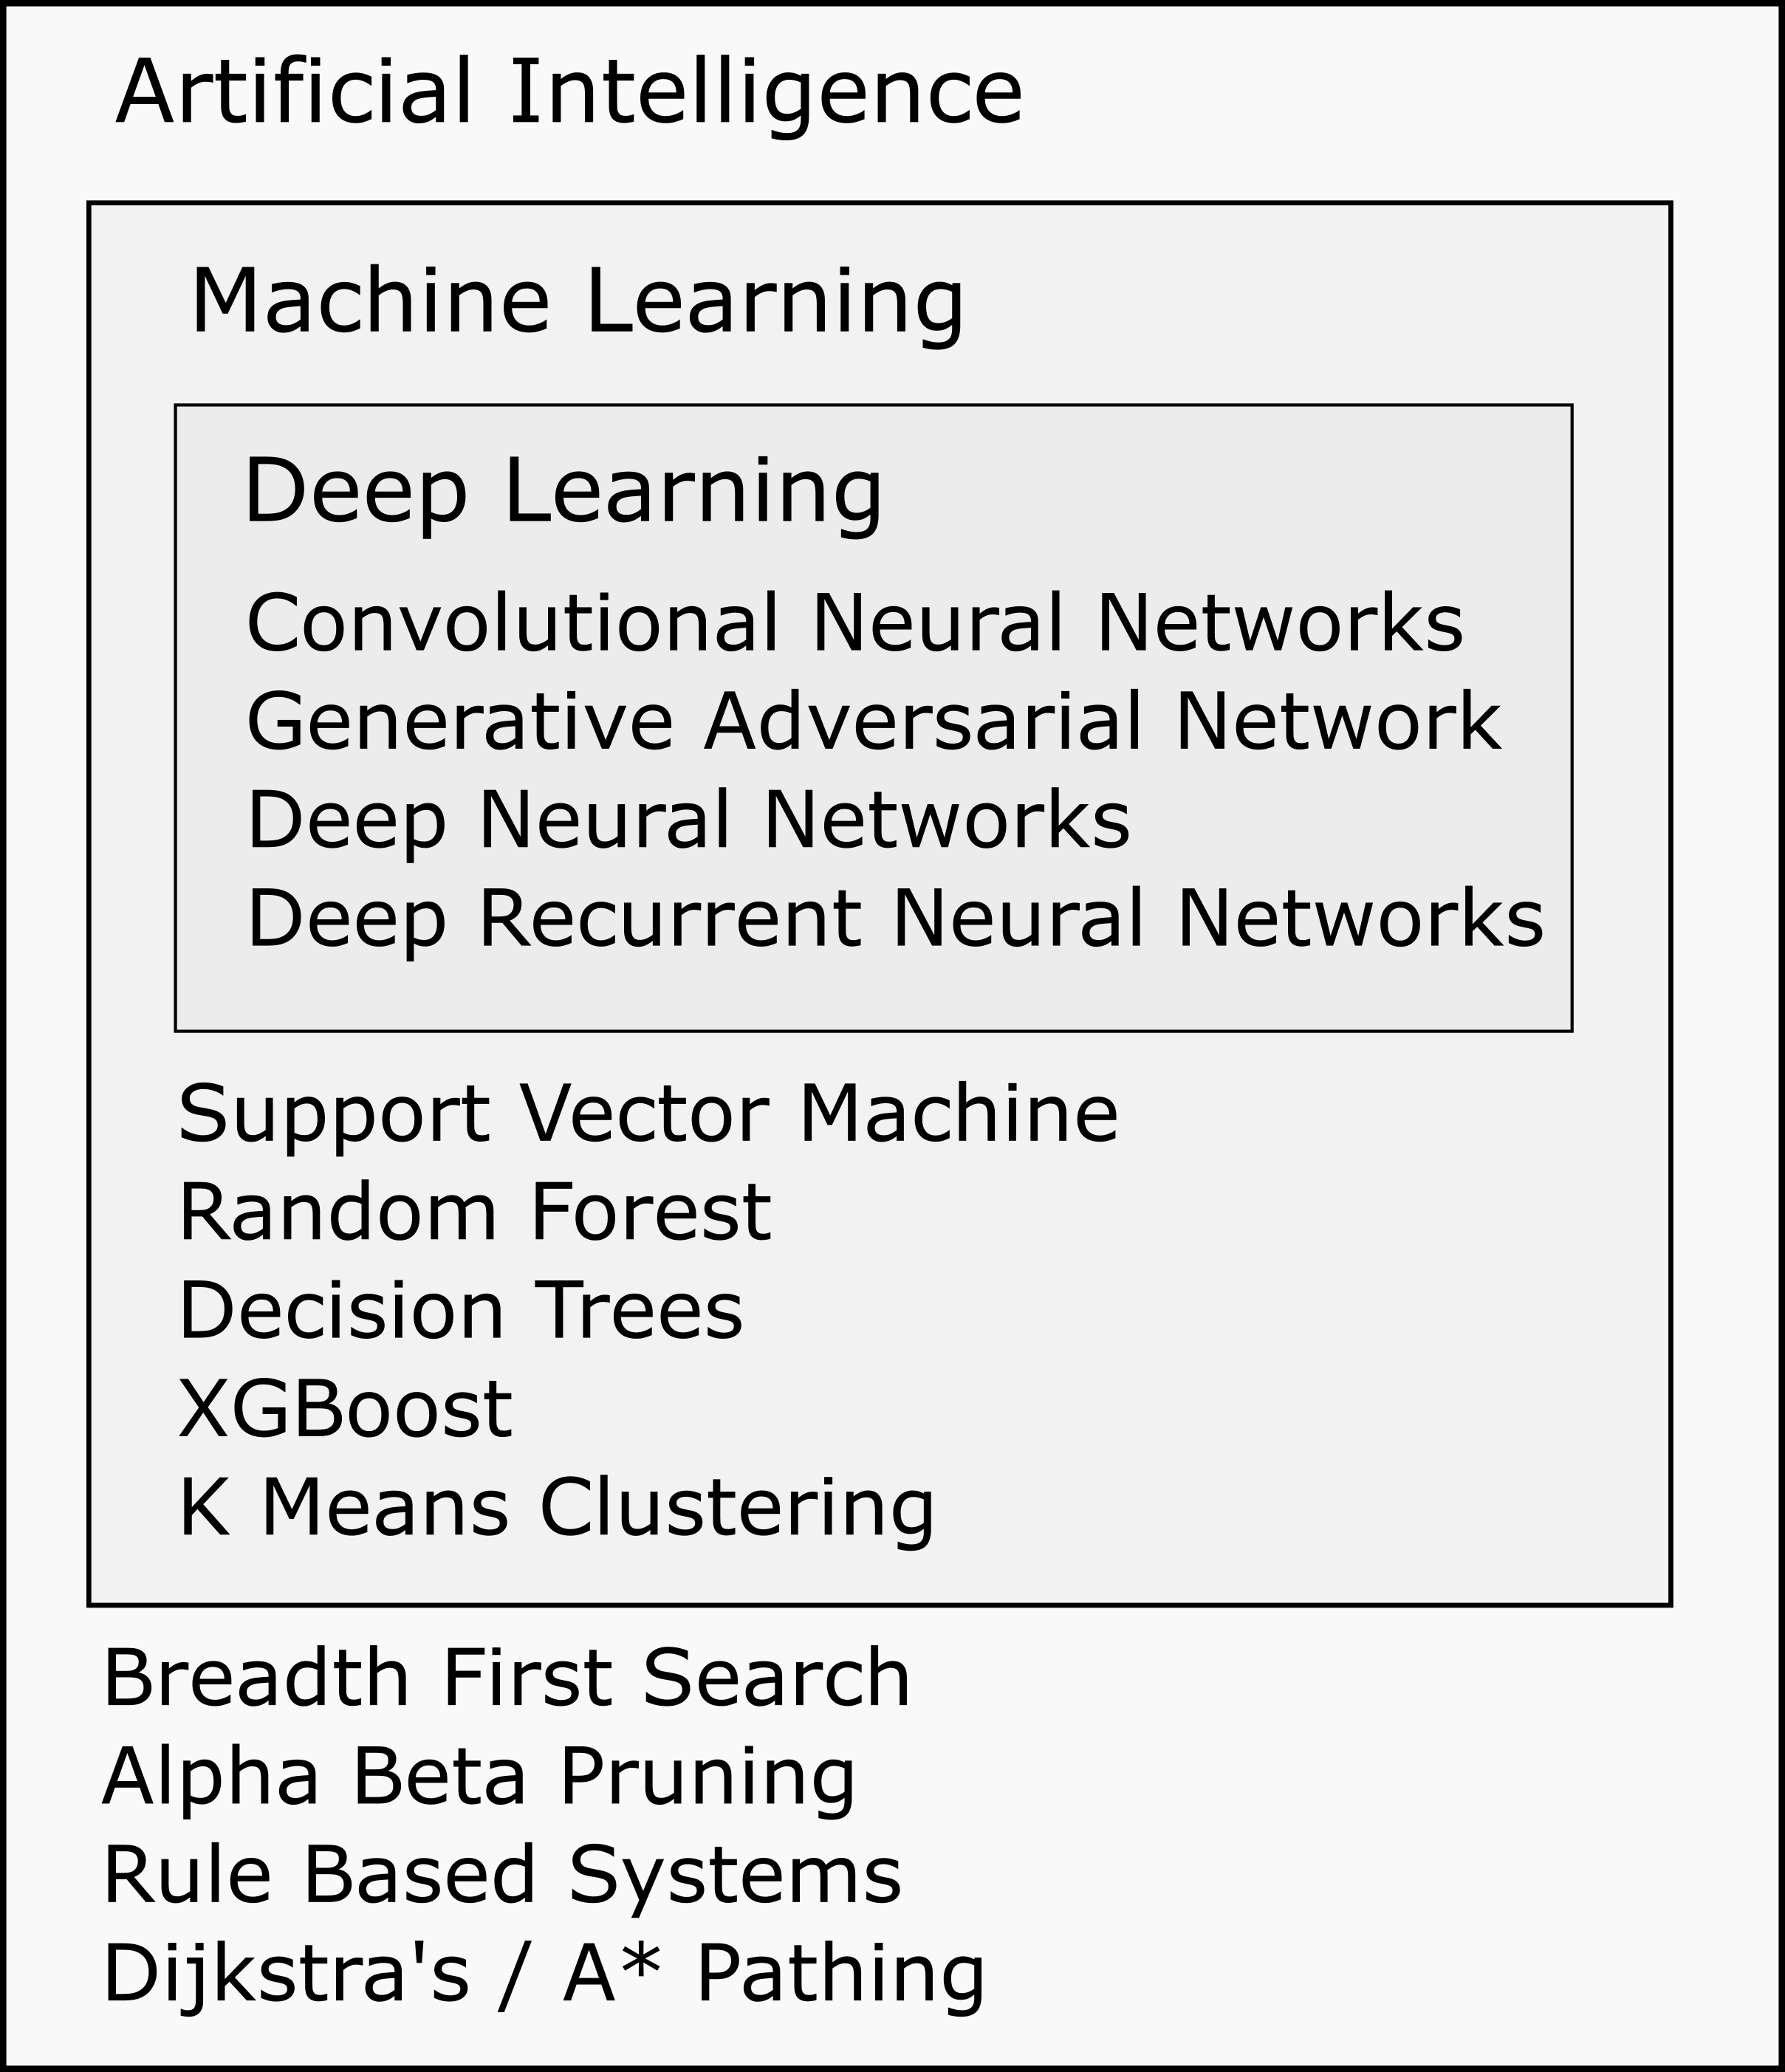
\includegraphics[width=60mm]{figs/ai_ml_dl.png}
    \caption{The fields of \gls{ai}, \gls{ml} and \gls{nn}, with examples of techniques in each.}
    \label{fig:ai_ml_dl} 
\end{wrapfigure}

%\end{SCfigure}

% link between perceptron and logistic regression clarified
% https://stats.stackexchange.com/questions/162257/whats-the-difference-between-logistic-regression-and-perceptron
Figure \ref{fig:ai_ml_dl} shows the relationship between \gls{ai}, \gls{ml} and \gls{dl}. \gls{ai} concerns the broad field of using technology to mimic human behaviour.\gls{ml} additionally involves training algorithms to find rules automatically based on training data, which can involve techniques usually situated within statistics, such as linear or logistic regression. \gls{dl} takes this a step further, concern the use of multi-layered \gls{nn}s trained on a large pool of training data to perform even more complex tasks, such as image segmentation or video captioning. The roots of \gls{ai} goes to the 1940s and 50s, with one particular event, the Dartmouth Summer Research Project, gaining particular retrospective notoriety for proposing to making significant advances in the field in a \enquote{2 month, 10 man study}  \cite{dartmouth_summer}. From a statistical perspective, using \gls{nn}s falls within the \enquote{algorithmic modelling} camp, as elaborated by Leo Breiman in \cite{two_cultures}. The emphasis is on predictive accuracy, not finding a data model.

\section{Machine Learning}
% name drop kernel trick

\gls{ml} is an interdisciplinary field at the intersection of mathematics, computer science and statistics and itself is often considered as a sub-field of the broad area of study that is  \gls{ai}. \gls{ml} deals with the challenge of "learning" from data without manual human input. In contrast to many statistical techniques, \gls{ml} is well suited to scenarios where predictive accuracy is paramount, training examples are both numerous and high dimensional, and inferential understanding is not critical [ZAMBINGO]. \gls{ml} gathered a lot of momentum in the 1990s, with the term \enquote{data mining} often used as a pseudonym. Traditional techniques in the field of \gls{ml} include decision trees,  \gls{svm}s (1992, \cite{svm}, K-means clustering (1962 \cite{k_means}, Naive Bayes and  \gls{flda}.  \bigskip

% probably delete this line 
Examples of classic data sets in \gls{ml} refer to unsupervised classification of data points into flower species, predicting diabetes risk based on a small subset of predictors, predicting whether a mine is present based on hundreds of frequency reflection variable and other challenges \cite{uci_ml_data}. Practical milestones include the use of Yan Le Cun's \enquote{LeNet} architecture in the late 1990s to perform accurate handwriting recognition. 

%At one stage, this algorithm (a \gls{cnn}) was responsible for the majority of automated cheque processing in the United States [ZAMBINGO].  \bigskip

The key idea is that the algorithm automatically finds and determines a set of rules to effectively label the input data based on some learning process that seeks to find the optimal set of model parameters. This avoids, for example, algorithms that are highly task specific (such as searching algorithms or algorithms specifically designed to find the optimal move given a particular rule set). \bigskip

\section{Neural Networks} 

% ZAMBINGO - mention hebbian learning

% ZAMBINGO - add page citation for linear combiner -> nn
\gls{nn}s (in this work, networks, \gls{ann}s and \enquote{nets} all refer to \gls{nn}s) started with the linear combiner, which with the addition of extra neurons, become the single-layer perceptron (also known as a single layer \gls{ffnn} \cite{haykin}. In a multiclass classification context, on the output layer of the perceptron, for each class we have a neuron $i$ which acts as the linear classifier $h_1, h_2, h_3, ... , h_i$. With the addition of a \gls{hiddenlayer}, this evolved onto the \gls{mlp}. Later, multi-layer \gls{ffnn}s were used, and the the architecture diversified into the \gls{cnn}s with the use of local receptive fields. A timeline of developments and architectures is present in figures \ref{fig:timeline_new_nn} and \ref{fig:timeline_old_nn}. \bigskip

\begin{figure}
    \centering
    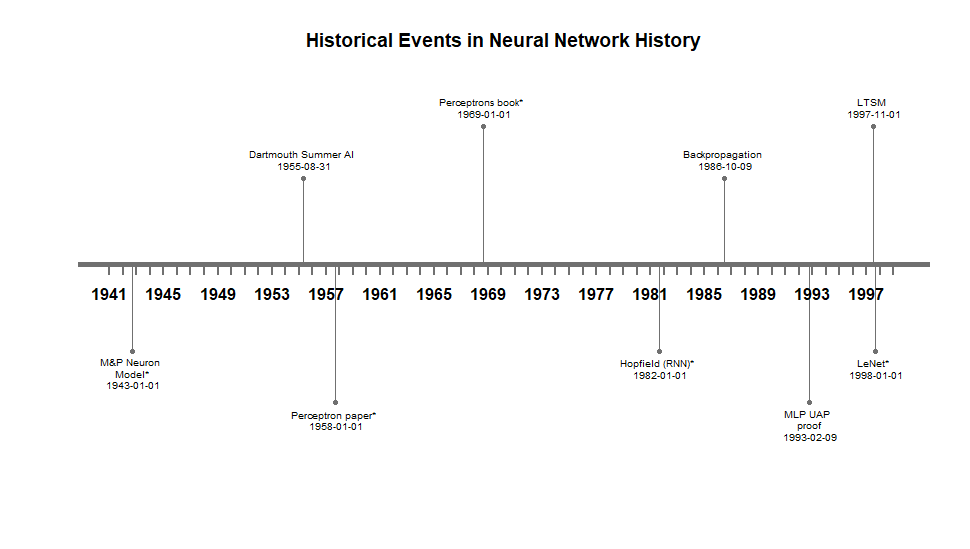
\includegraphics[width=140mm,scale=1.5]{figs/timeline_old_nn.png}
    \caption{A selection of events in early neural network history}
    \label{fig:timeline_old_nn}
\end{figure}

\begin{figure}
    \centering
    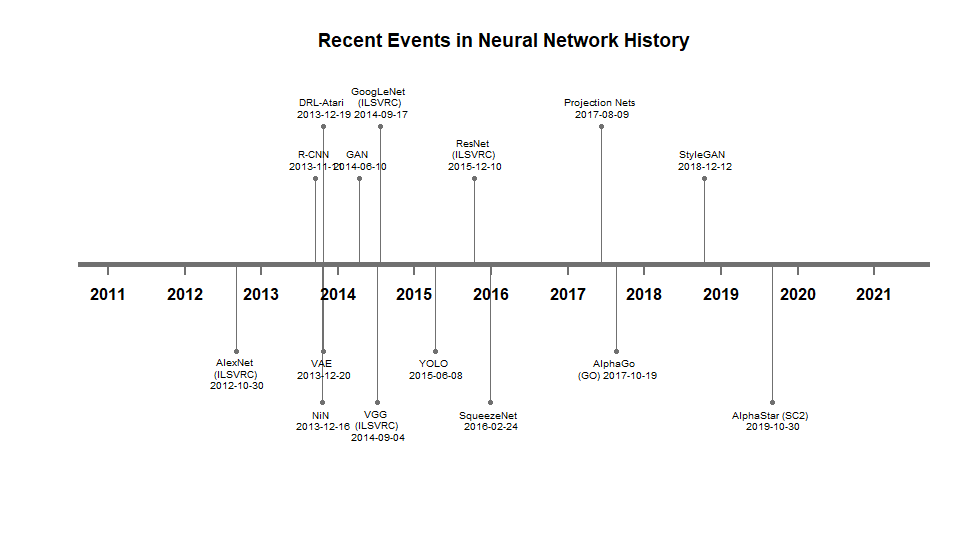
\includegraphics[width=140mm,scale=1.5]{figs/timeline_new_nn.png}
    \caption{A selection of events in modern neural network history}
    \label{fig:timeline_new_nn}
\end{figure}

Figures \ref{fig:timeline_old_nn} and \ref{fig:timeline_new_nn} show a small selection of key historic and recent events. To help map out the labyrinth of architectures developed over time, figure \ref{fig:nn_architectures} shows some \gls{nn}s and the key influences.

% Zambingo - DiagrammeR R
%\begin{figure}
%    \centering
%    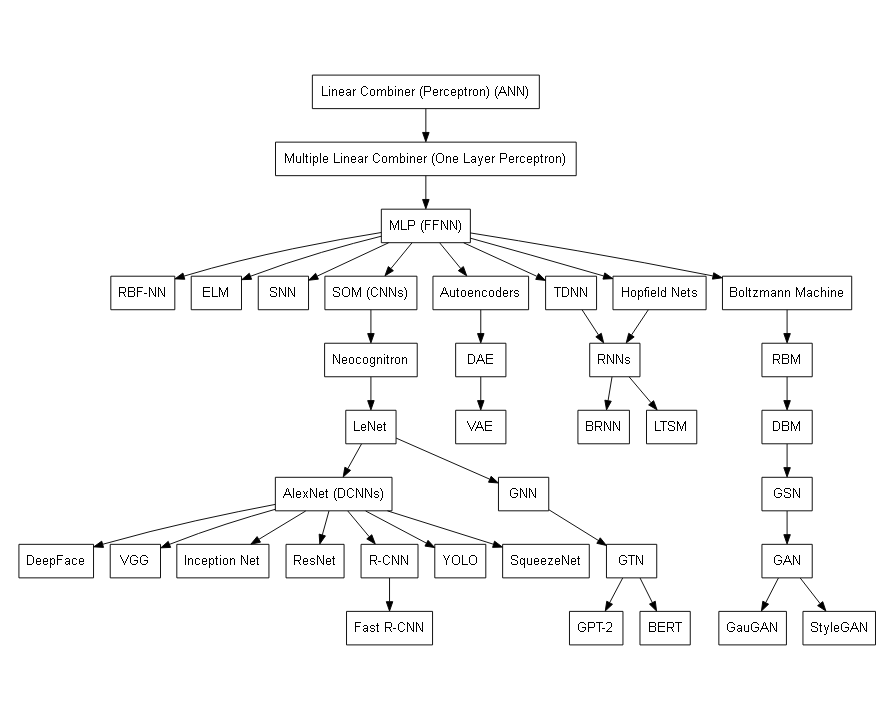
\includegraphics[width=140mm,scale=1.5]{figs/nn_architectures.png}
%    \caption[Neural network architectures.]{A small selection of the key historic and %modern \gls{nn} architectures leading up to the present day, with the relationship %to their key influences shown.}
%    \label{fig:nn_architectures}
%\end{figure}

A \gls{nn} can be interpreted many ways. For example, a common interpretation is that \gls{nn} act as function approximation machines, a view influence by the \gls{uap} theorem for \gls{mlp}s, which states that;

\begin{quote}
    A standard multilayer feedforward network with a locally bounded piecewise continuous activation function can approximate any, continuous function to any degree of accuracy if and only if the network's activation function is not a polynomial.\cite{uap_mlp}
\end{quote}

Another view of \gls{nn}s is as an extremely simply approximation of how the brain works. This has more of a parallel when the heaviside activation function, where, if the input signals of the neuron (the weighted attributes of the \gls{instance}, which can be thought of as analogous to the dendrites of a neuron) surpass a given threshold, the neuron \enquote{fires}, sending an output signal down the axon (i.e. returns a one, instead of zero).
\bigskip

At it's simplest a \gls{nn} for binary classification is a single \gls{neuron} comprising of a weighted sum of the input features, the addition of a bias term and the application of an \gls{activationfunction} to provide an output for a given input \gls{instance} $i$. This is summarised in \ref{fig:nn_simple} \footnote{\href{https://playground.tensorflow.org/}{Interactive Example of \gls{nn}s, hosted by TensorFlow.}}.  

\begin{figure}
    \centering
    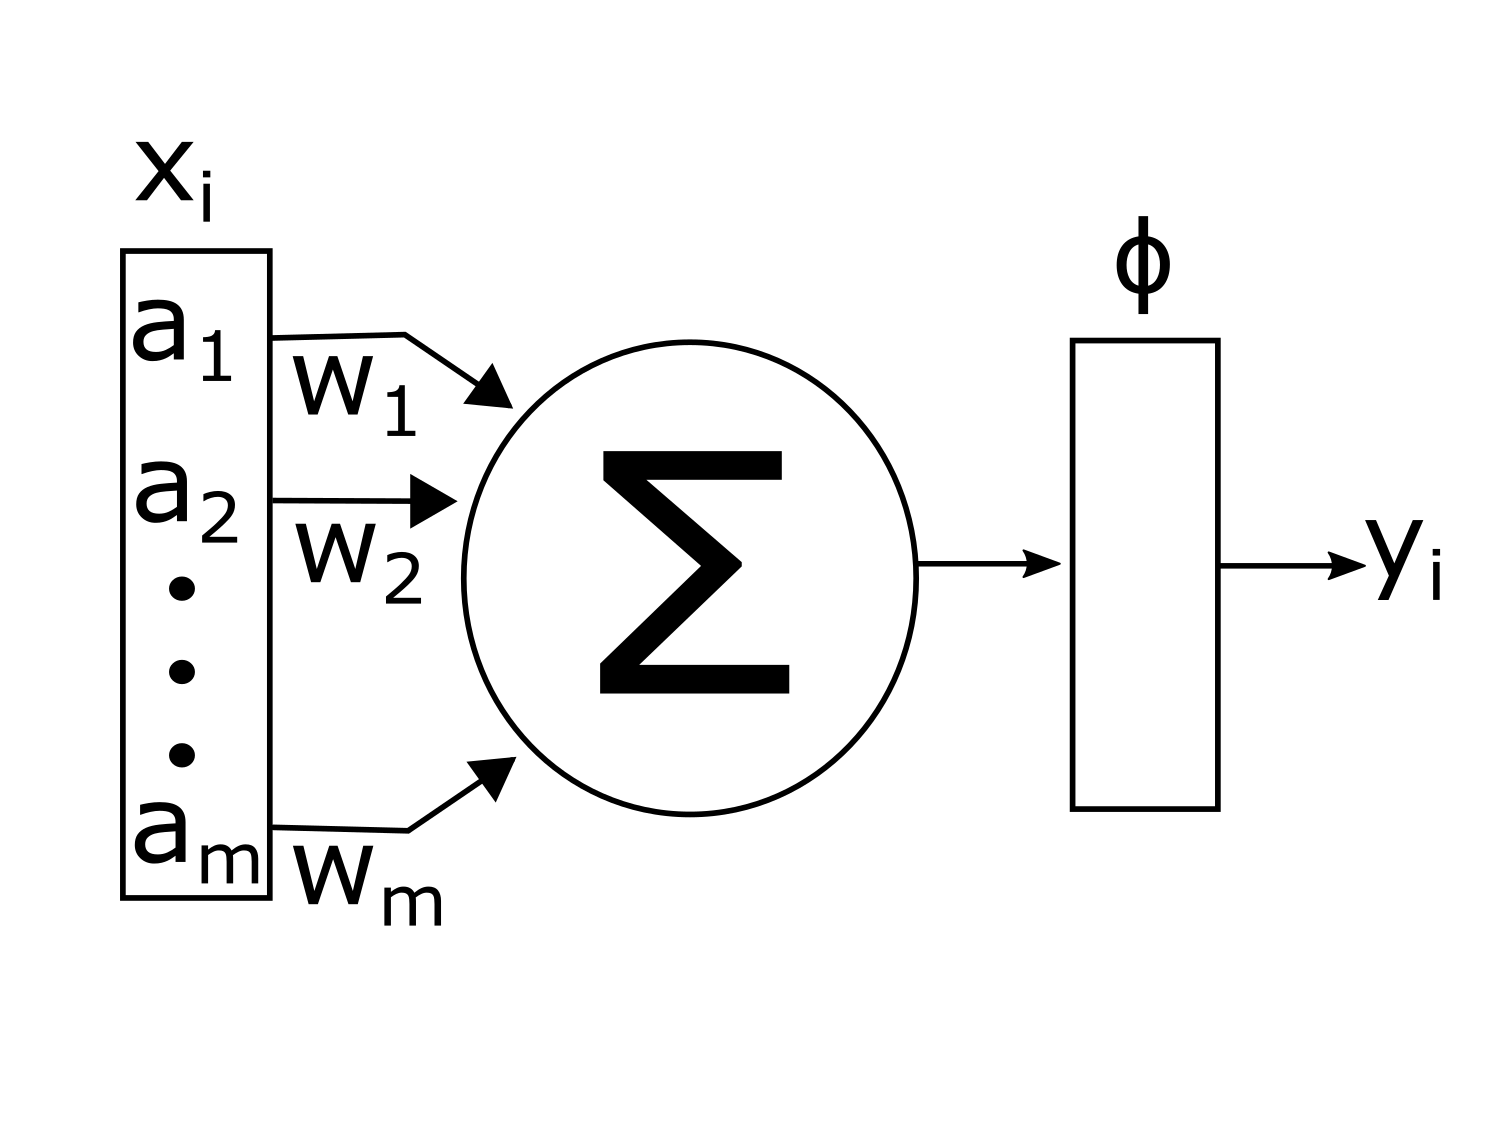
\includegraphics[width=100mm]{figs/nn_simple.png}
    \caption{The prediction process for a single point of data in a linear combiner.}
    \label{fig:nn_simple}
\end{figure}

\begin{equation}
    y_i = \mathds{1} ((\sum_{j = 1}^m w_j + b_m) > 0)
    \label{eq:nn_simple_pred}
\end{equation}
%\myequations{Prediction for a Linear Combiner}

This network is a binary \gls{linearclassifier}, which has a single \gls{layer} and uses the heaviside \gls{activationfunction} (figure \ref{fig:heavi_function}) and does not use a bias term (would would be added to the weighted sum). The output $y_i$, can be either a one, or a zero. It therefore has a single parameter for each non-class attribute present in the input data, which corresponds to each weight, $w_m$. Choosing an \gls{activationfunction}, $\phi$ when designing networks in modern times often comes down to using the \enquote{tried and true} functions (such as \gls{relu}), or a lot of manual \gls{hyperparameter} tuning.

\begin{wrapfigure}{l}{0.5\textwidth}
    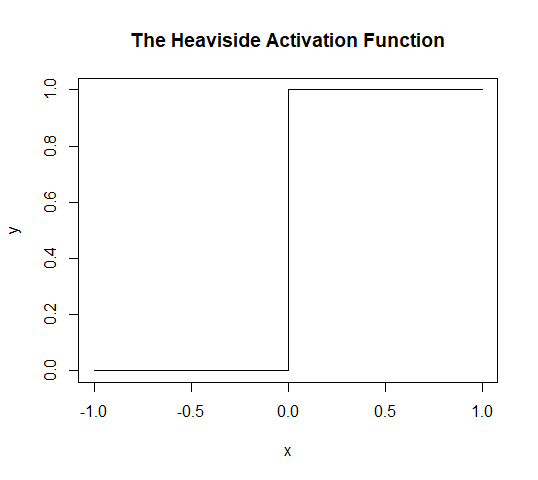
\includegraphics[scale=0.5]{figs/heavi.png}
    \caption{The Heaviside activation function.}
    \label{fig:heavi_function}
\end{wrapfigure}

% spiel about VC dim and linear classifiers using simple logistic regression (and link to NN)
If we use the sigmoid \gls{activationfunction} and incorporate a bias term, we now have what is equivalent to a logistic regression. Hence there is a parallel that can be drawn between a particular configuration of the perceptron, an early technique in \gls{ml} and the traditional statistical logistic regression. By a running a logistic regression with data that has the minimal \gls{vc} dimension (3) for a \gls{linearclassifier}, we can see that the classifier can always \enquote{shatter} (perfectly separate) the data. This is because the \gls{vc} dimension of a linear classifier is $d+1$. However, if we increase the number of points to four (surpassing the \gls{vc} dimension of the classifier), we now find this is not always true (see figure \ref{fig:vc_4}).

\begin{figure}[H]
    \centering
    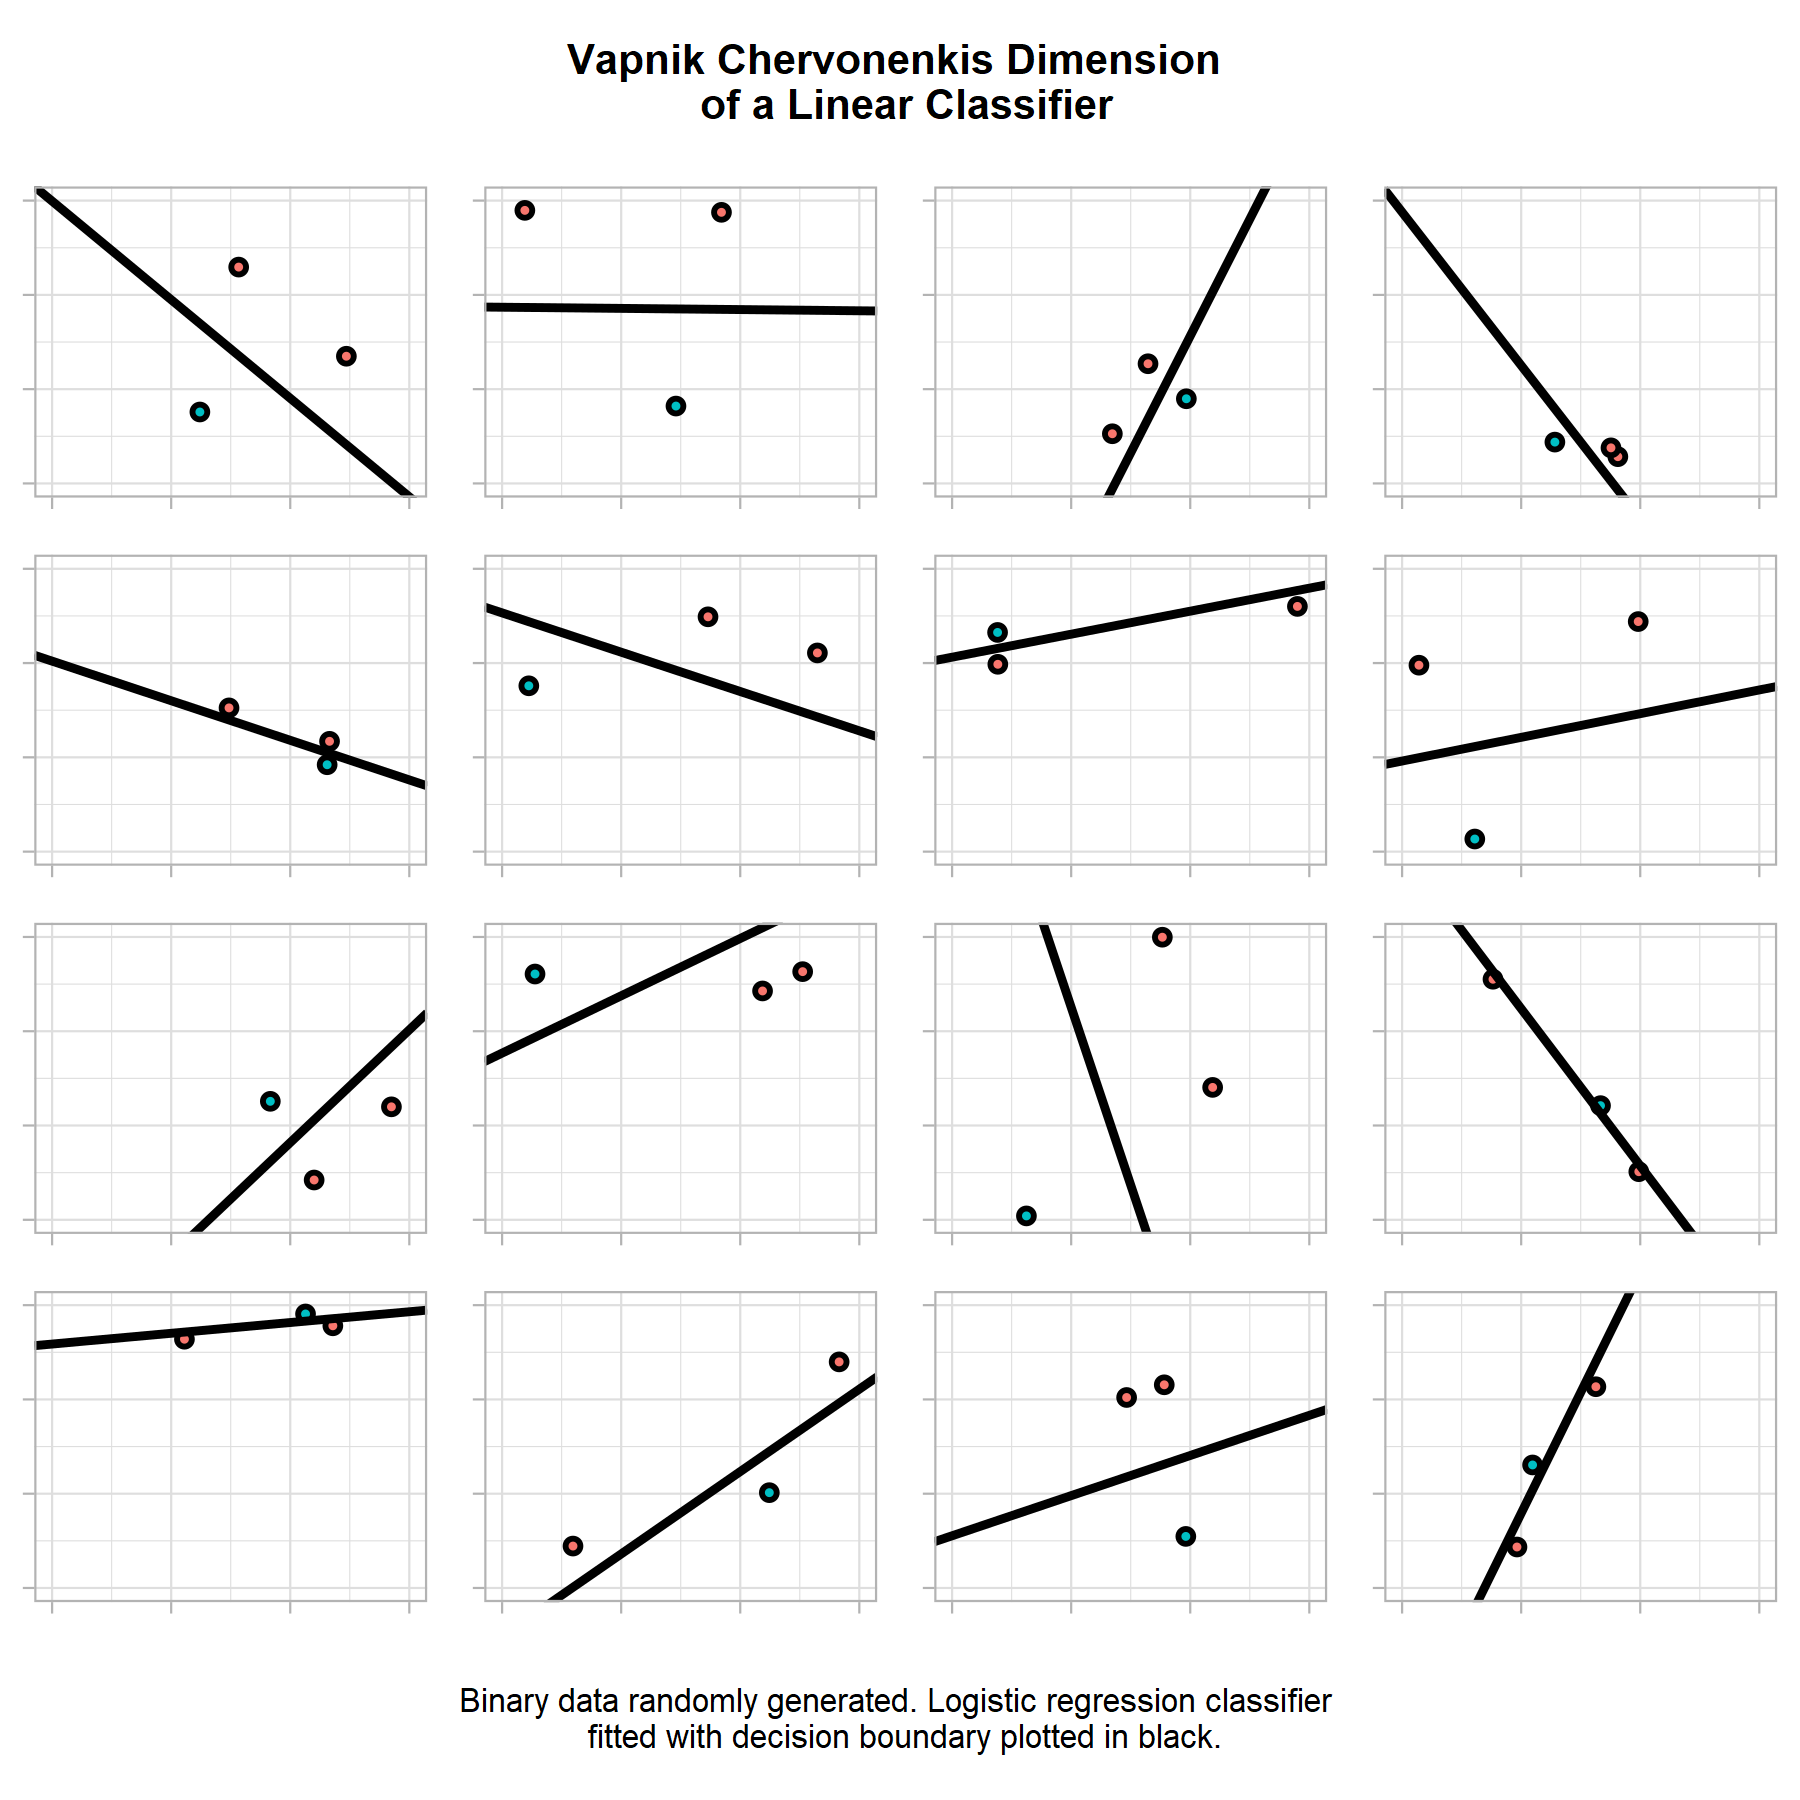
\includegraphics[width=120mm]{figs/vc_3.png}
    \caption[\Gls{vc} dimension of a linear classifier - the data is shattered.]{In two dimensions, logistic regression (a linear classifier) can perfectly shatter a data set with three points, in all cases. The points have been randomly generated in each plot, a logistic regression fitted to each data set using $x, y$ as covariates.}
    \label{fig:vc_3}
\end{figure}

\begin{figure}[H]
    \centering
    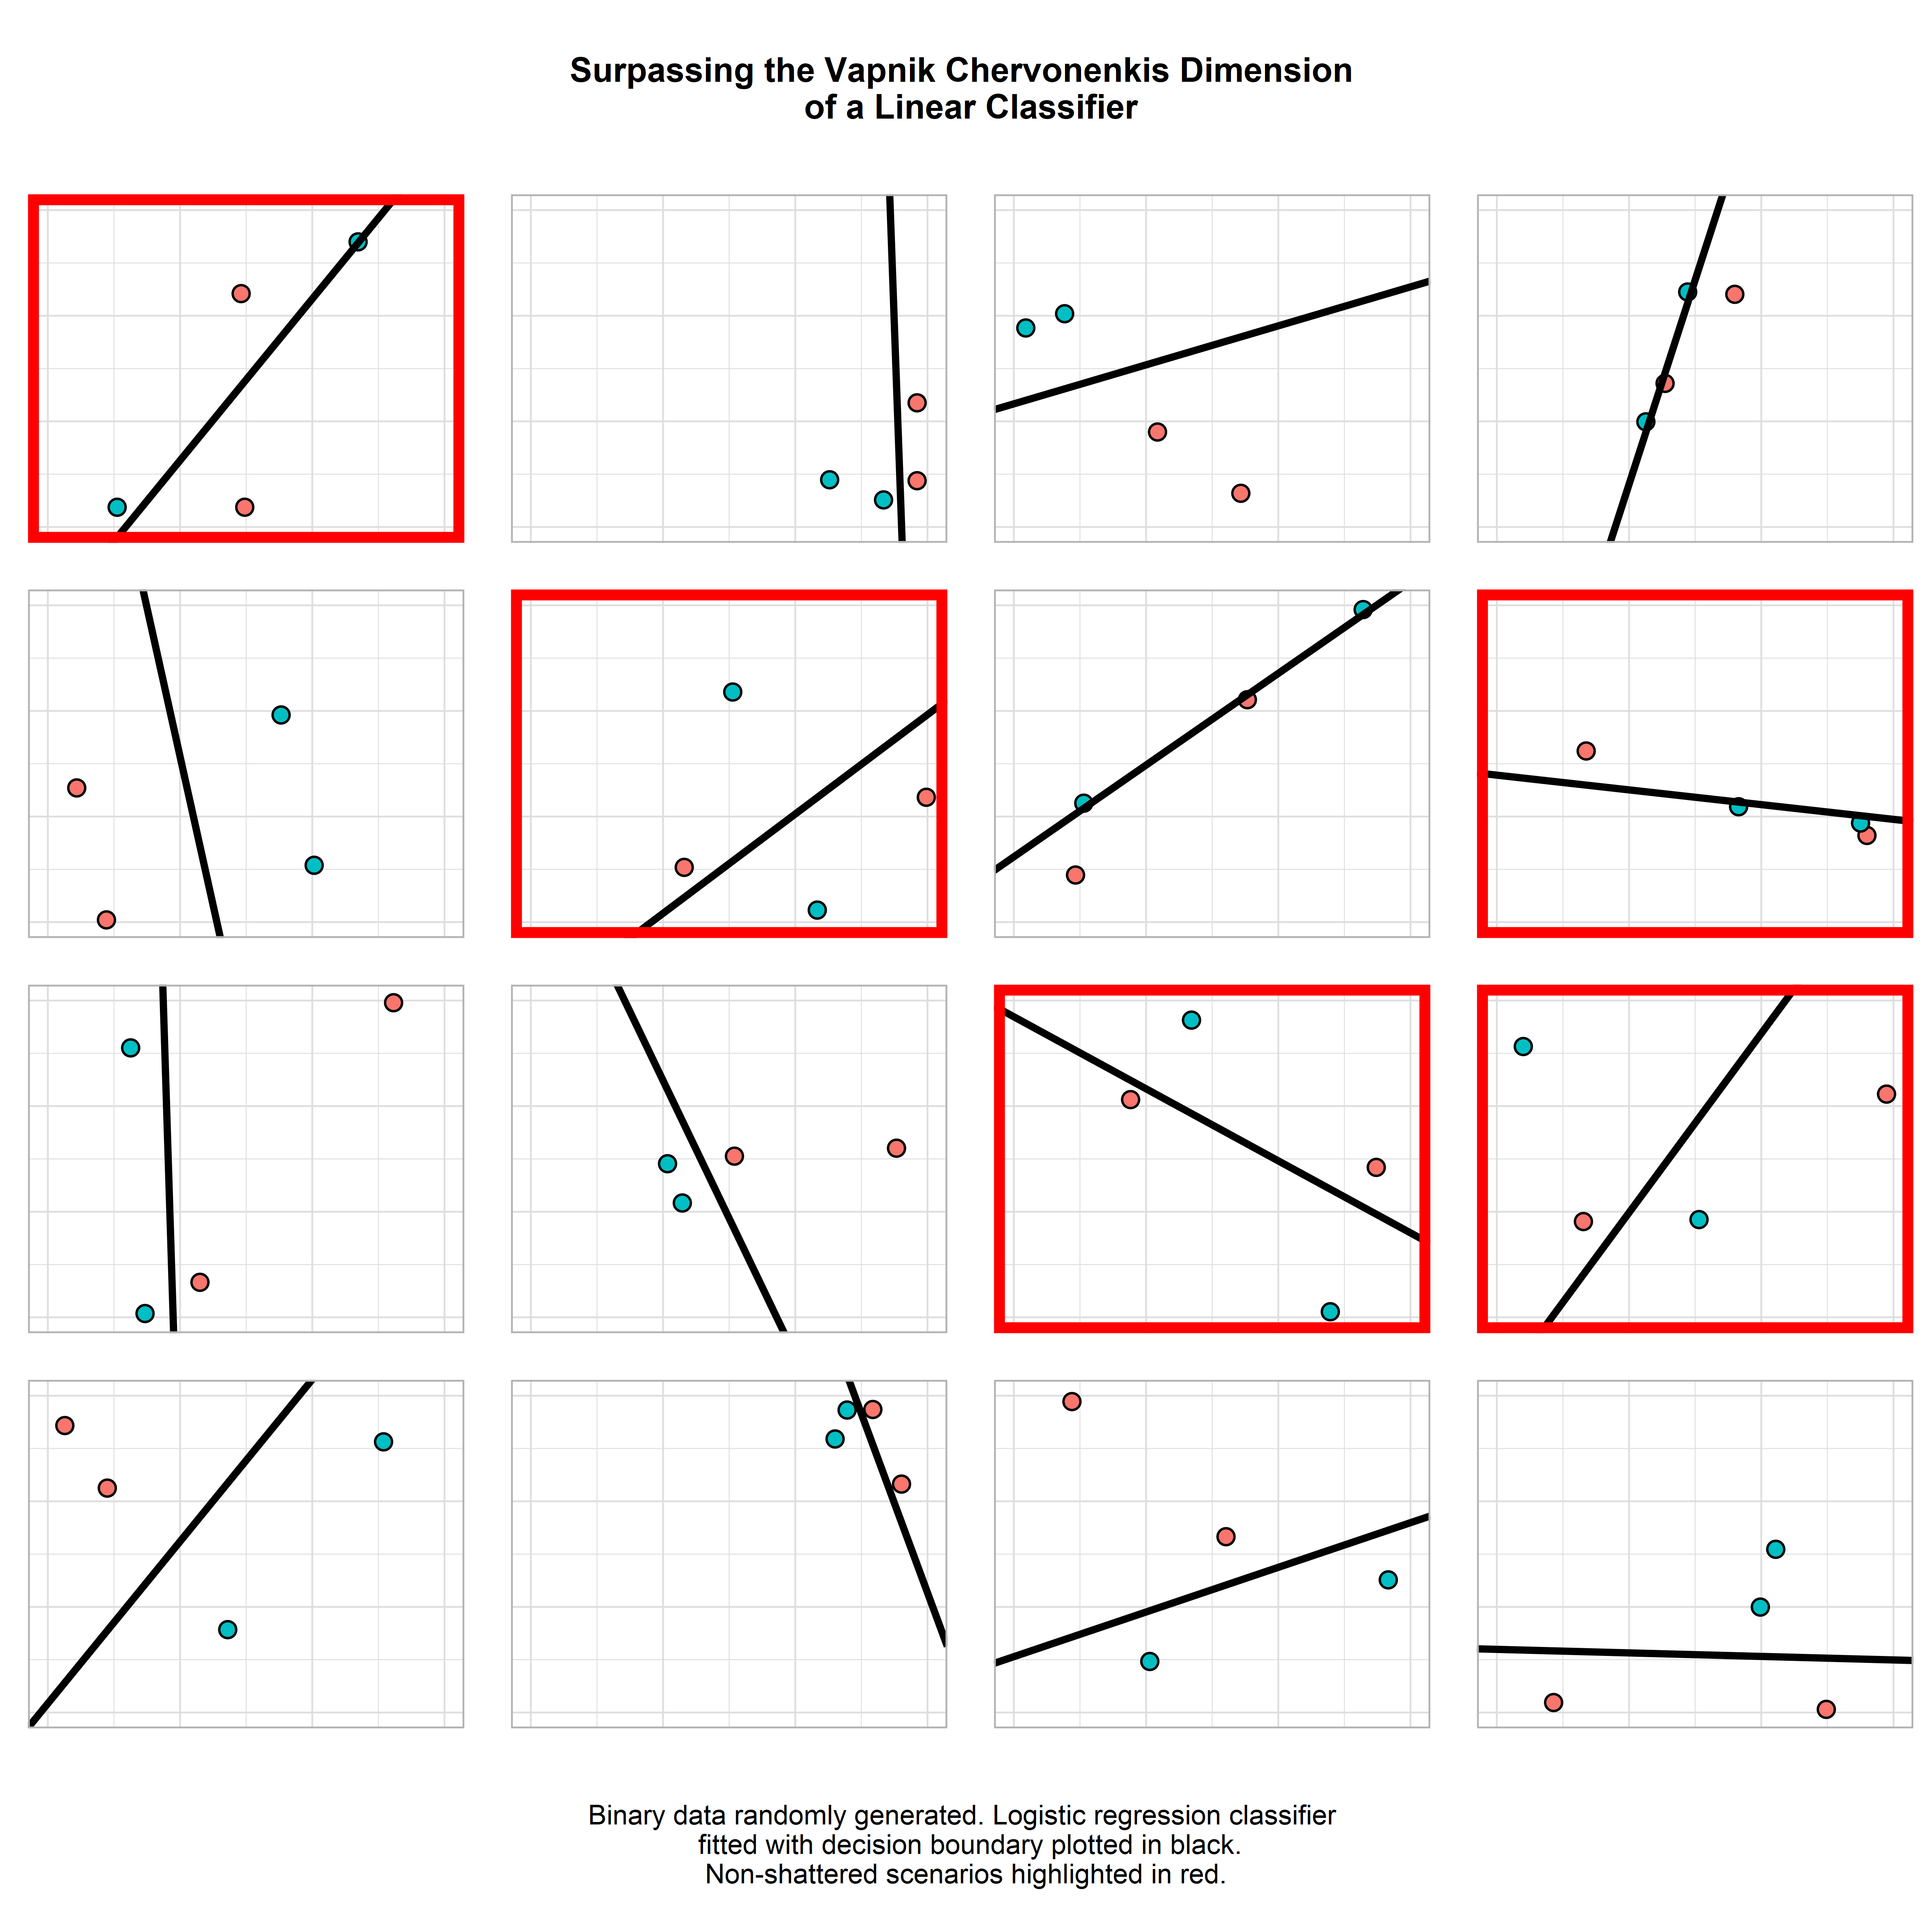
\includegraphics[width=120mm]{figs/vc_4.png}
    \caption[Surpassing the \gls{vc} dimension of a linear classifier - the data is not always shattered.]{\Gls{linearclassifier}s begin to falter once the VC dimension of the classifier is surpassed in the data. The points have been randomly generated in each plot, a logistic regression fitted to each data set using $x, y$ as covariates and the plots are set to automatically highlight instances of imperfect separation of the data.}
    \label{fig:vc_4}
\end{figure}

\begin{wrapfigure}{l}{0.5\textwidth}
    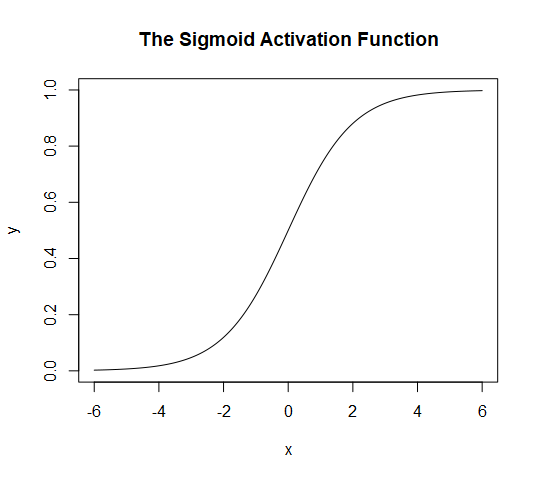
\includegraphics[scale=0.5]{figs/sigmoid.png}
    \caption{The Sigmoid activation function.}
    \label{fig:sigmoid_function}
\end{wrapfigure}

Many \gls{nn} diverge from most statistical techniques in that they do not assume a distribution over the data, rather taking an \enquote{algorithmic} approach to classification and prediction \cite{two_cultures}. They leverage the increased classifier complexity that results from the addition of extra neurons to layers (\enquote{going wide}) and the addition of \gls{layer}s (\enquote{going deep}). This increased complexity comes at the cost of the interpretability, although a variety of techniques are in development to address this problem \cite{nn_interpretability}. Basic uses of \gls{nn}s include statistical pattern recognition, temporal pattern recognition and image recognition (e.g. using \gls{ffnn}s, \gls{rnn}s and \gls{cnn}s, respectively).

\gls{nn}s find their origins in the fields of psychology and electronic engineering, dating back to the days of linear adaptive filters in the \cite{haykin}. This began perceptron model proposed by Rosenblatt \cite{perceptron_paper} as an extension of the McCulloch and Pitts model of the neuron \cite{logical_calculus} \bigskip
% ZAMBINGO - figure idea - branching tree of nn architectures leading to cnns

% REDO DIAGRAM IN GGPLOT2
\begin{figure}
    \centering
    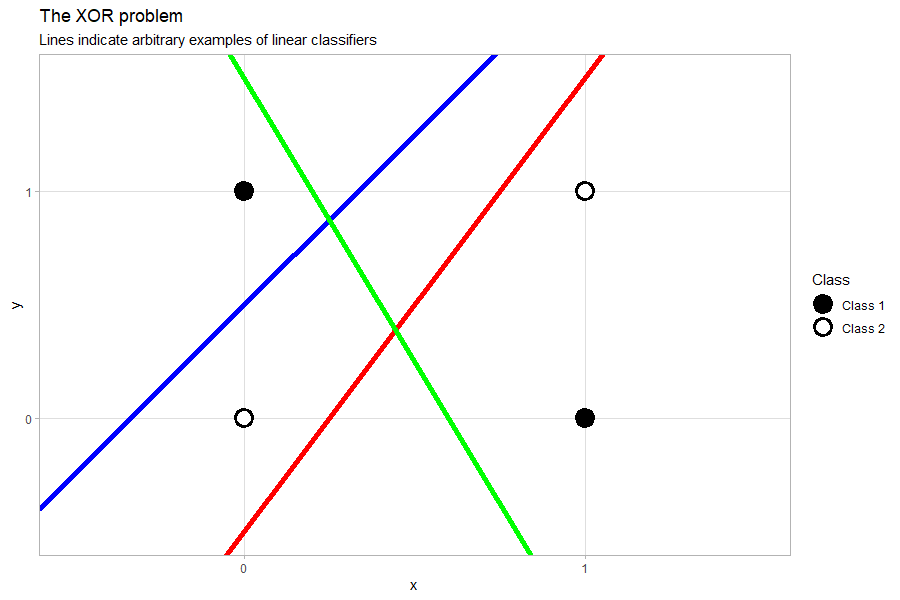
\includegraphics[width=120mm]{figs/xor_problem.png}
    \caption[The \gls{xor} problem]{An illustration of the \gls{xor} problem that a perceptron can not solve. Lines indicate arbitrary examples of \gls{linearclassifier}s.}
    \label{fig:xor_problem}
\end{figure}

% Zambingo - would be good to add reference for popularity of book
The \gls{xor} problem is the simplest possible example of data that is not \gls{linearlyseparable}, and thus not able to be classified using a \gls{linearclassifier}. One milestone was when the highly influential book,\enquote{Perceptrons} proved that the \gls{xor} problem (figure \ref{fig:xor_problem}) could not be solved with a single layer perceptron \cite[Chapter~4]{perceptron_book}. However, \gls{mlp}s and kernel perceptrons are able to solve this problem. Interest in \gls{nn}s died off considerably in the 1970s/80s - this is often referred to as the \enquote{AI winter} \cite{ai_winter}. This continues to cause general speculation around whether another such \enquote{winter} will occur \cite{ai_winter_spec}.  \bigskip

% Can't seem to find a reference for this.
%It has been speculated \cite{perceptron_spec} that this was in part because the idea %that \gls{mlp}s could not solve the \gls{xor} problem gained traction, despite the %authors acknowledging that it was likely that they could in their book %\cite{perceptron_book}.

% This culminated in a general decrease in funding and a shift in focus, with leading conferences in the field, such as \gls{nip}s receiving more submissions under the field of data mining than \gls{nn}s, despite being explicitly a conference centered around neural systems

Eventually however, research with layered \gls{nn}s intensified and progress was made, not least in part because of advances in computational power;

\begin{quote}
...the IBM 704 computer that cost \$2 million in 1958, or \$20 million in today’s dollars, could perform 12,000 multiplies per second, which was blazingly fast at the time. The much less expensive Samsung Galaxy S6 phone, which can perform 34 billion operations per second, is more than a million times faster...\cite{unreasonable_dl}
\end{quote}

\bigskip
Coming out of the AI winter, \gls{nn}s were restricted to four or five layers (never past ten). There was a \enquote{node budget} and a lot of manually configured architecture at the node level. The manually specified architecture of the network was critical to it's success \cite{manual_architecture}, for example in computer vision, where significant amounts of feature engineering was required. 
\bigskip

% ZAMBINGO - need to find citation for this
%In 1997, Yan Le Cun developed the first neural network capable of high accuracy digit %recognition which outperformed the previously popular \gls{svm} models. \bigskip

% CNN

\section{Deep Learning}

% ZAMBINGO - reference for AI safety would be good here - parameter space, understanding of bounds etc

Highly layered ("deep") \gls{nn}s lie at the heart of \gls{dl} and are in fact all extensions of the \gls{mlp}. The phrase \enquote{deep} has a level of subjectivity around it; clearly, a two \gls{layer} \gls{mlp} is not a \gls{dnn}, but is a 5-layer network \enquote{deep}? The most Other deep algorithms do exist (such as \enquote{deep trees} \cite{deep_forest}) although these are unable to handle complex image classification problems as well as other modern {dnn}s. \gls{dl} is seen as a highly effective strategy in a variety of \gls{ai} applications. As a model, they are far more complex than most statistical models, having millions of parameters \cite{unreasonable_dl}.  
\bigskip
% AI winter mention and comeback - LeNet CNNs then cooling SVMs

Practical achievements (figure \ref{fig:timeline_new_nn}) include progress made in \gls{drl}, such as teaching a network to effectively play a variety of Atari games without any manual intervention \cite{drl_atari}. \gls{cnn}s have been built on to apply artistic filters to images \footnote{\href{https://deepart.io/}{Interactive example here.}} using style representations \cite{neural_style}. Generative networks progressed, with the development of \gls{vae}s, which could generate examples from complex distributions and were then surpassed by the development of \gls{gan}s for the generation of highly realistic examples \cite{gans}\footnote{\href{http://www.whichfaceisreal.com/index.php}{Try this website as an interactive example.}}. AlphaStar \cite{alphastar} and AlphaGo \cite{alphago} gained a lot of attention \cite{press_alpha_go} \cite{press_alpha_star} for beating top human players in the board game Go and the video game StarCraft II. In the later case, the \gls{ai} was constrained in terms of \gls{apm}, it's view and a realistic observation delay and network latency. Both games are notably complex with the first having an extremely large state space (having a search space of $10^360$ moves, versus $10^{43-123}$ for chess \cite{moves_chess_go}) and the second having a complex continuous real time state space, often requiring  around hundreds \gls{apm} for top human players. Style\gls{gan}s were notable for even higher degrees of realism, which was also picked up in the media \cite{press_stylegan}.
\bigskip

In terms of \gls{cnn}s, kicked off a flurry in research activity in \gls{dl}, as it was the first \gls{dnn} to win the \gls{ilsvrc}, in 2012 \cite{alex_net} \cite{dl_overview}. \gls{r-cnn}s were notable for classification of regions and \gls{semanticsegmentation} using \gls{cnn}s. \enquote{GoogLeNet} introduce a more parallel architecture with the \enquote{inception} module to achieve higher accuracies \cite{googlenet}. \gls{resnet}s broke new ground with it's extreme depth \cite{resnet} by surpassing \enquote{human level recognition} (\cite{resnet_human}, Section 6.4). \enquote{SqueezeNets} introduced high performing \gls{cnn}s with far fewer parameters and a smaller memory footprint \cite{squeeze_net}. 
\bigskip

For context \gls{nn}s had now significantly fallen out of favour [ZAMBINGO] and \gls{svm}s were rapidly gaining popularity \cite{svm_nn_comparison}. This trend continued until 2012, when the striking performance of AlexNet, a \gls{dcnn}, in the influential annual \gls{ilsvrc} created a lot of interest in practical achievements of \gls{dl} in the image recognition space. The remarkable improvements in performance achieved showed the viability of \gls{dl} as an alternative to \gls{svm}s and other techniques, for \gls{imagerecognition}. This demonstration was enabled by several factors contributing to recent rapid developments in \gls{dl}: the availability of \gls{dl} tool-kits, such as Theano and Caffe (2007, 2013 - REF), and Keras, TensorFlow and PyTorch (2015, 2016 ZAMBINGO); advances in computational hardware and accessibility, including powerful purpose-built \gls{gpu}s, access to cloud compute (\gls{aws}, \gls{gcp}, Azure, \gls{tpu}s) and decreasing cost barriers (Google Collab, MatrixDS, note on costs e.g. declining storage costs); and access to large, curated data sets for training (large text corpuses \cite{enron_emails}, image repositories \cite{image_net}) \bigskip

Now, \gls{nn}s can be incredibly deep, from 50 to over a thousand layers (depths used with \gls{resnet}s \cite{resnet}) and also quite wide (for example, \gls{elm}s that have a single layer, but are hundreds or thousands of neurons wide). Going deep, however, seems to be associated with the extraction of semantics at progressively more abstract levels (\cite{cnn_semantics}). 
\bigskip

% insert summary table of models used in ILSVRC, number of parameters, hardware trained on, architecture, unique features and top 1/3/5 accuracy's

% when to capitalise fields?
While this was a major advancement for \gls{dl} in the problem domain of image classification, progress was being made in other domains such as speech recognition, handwriting recognition, image segmentation, image captioning and generative models \cite{dl_overview}. 
\bigskip % todo - finish list of progress in domains
 
\gls{dl} has evolved as a subset of \gls{ml} methods used for extracting complex semantics from data. \gls{dl} methods have achieved a wide variety of goals that would not otherwise be possible via traditional machine algorithms (such as realistic face generation \footnote{For an excellent example of this, see \href{https://www.thispersondoesnotexist.com/}{This Person Does Not Exist}, for realistic faces generated by Style\gls{gan}s})  \bigskip
% todo - finish list of goals 

The success of  \gls{dl} has fuelled the development of a plethora of different  \gls{nn} architectures, including \gls{ltsm}s, \gls{rnn}s and \gls{gan}s. These are now widely used in a variety of applications, such as for text-to-speech, handwriting recognition and art generation (respectively).  
\bigskip % Zambingo - need to add citation for applications (check review)

\section{Convolutional Neural Networks}

% Zambingo - add ref for neocognitron
\gls{cnn}s were inspired by the 'Neocognitron' of the 1980s \cite{neocognitron_proposal} \cite{neocognitron}. This was notable for having a concept similar to \gls{localreceptivefields} and a strategy similar to the pooling and covolution that occurs in modern \gls{cnn}s. \gls{cnn}s were developed in earnest by in the 1990s, with early uses involving reading cheques \cite{lecun_cheques}. The primary purpose of \gls{cnn}s is \gls{imagerecognition}, although they are also used in time series forecasting (1D \gls{cnn}s) and can be used for 3D recognition, for example using sensors from the Microsoft Kinect (\cite{3d_conv}). \gls{cnn}s hinge on 'local receptive fields' (also known as sparse connectively), which means that each of the input layer neurons have a particular patch of the input data that they connect to. The input data (or function) undergoes a convolution, in that a filter (or kernel) is convolved (slid across) the data. Each successive \gls{neuron} in a given layer \cite[Chapter~5]{good_fellow_2016}

% bit on how convolution works
% bit on pooling (or decimation)
% diagram of dimensionality through network

%removed "generally"

\section{Applications}

Image classification is a subset of the broader area of computer vision, which includes such applications as face , object, feature and landmark detection, feature detection, realistic  generation of class examples and art generation.  
\bigskip
%The field of \gls{dl} is a relatively modern one, and recent developments have been popularised through %making appearances in the media, through the striking use of neural style transfer to make various %surprising images or videos - such as the face of a dollar bill, speak a particular phrase, the Mona %Lisa come to life or even figures like Marilyn Monroe take the stage once more [ZAMBINGO]. 

The underpinnings of the resurgence of \gls{dcnn}s in recent times is linked to the use of \gls{dcnn}s for the ImageNet challenge. Prior to this challenge, \gls{dl} had was not widespread due to several problems; computational resources, sufficient training data, a lack of accessible tool-kits and the "vanishing gradients problem" \cite[Chapter~8]{good_fellow_2016} \cite[p.~93-94]{dl_overview}. Today, there is a wide breadth of techniques in \gls{dl}, from deep \gls{rnn}s for object detection in videos, \gls{gan}s for image and video generation, \gls{dcnn}s for \gls{imagerecognition}, ... 

%Recent major developments include Neural Ordinary Differential Equations

\section{Tools and Hardware}

Given the computational complexity of  \gls{dl} models, the providence of good tools has accelerated the development of algorithms. A selection of these tools a proxy for their popularity is shown in figure \ref{fig:git_stars}.

\begin{figure}
    \centering
    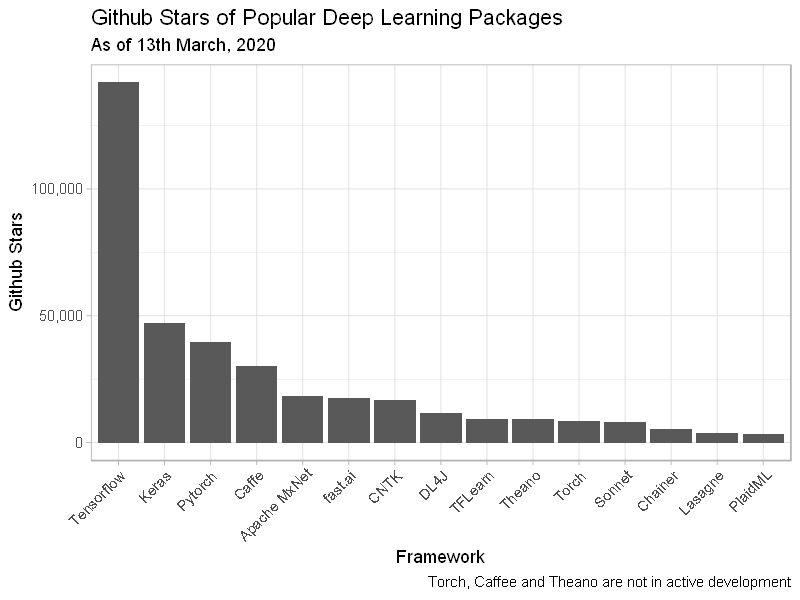
\includegraphics[width=120mm]{figs/gitstars.png}
    \caption[Popular \gls{dl} frameworks]{Common open source \gls{dl} frameworks as of March, 2020. Github stars are used a simple proxy for popularity.}
    \label{fig:git_stars}
\end{figure}

\gls{dl} tools started with Torch (2002), Caffe, Theano and a variety of disparate frameworks and later evolved into Pytorch, Keras and Tensorflow, which have become the main tools of research and production in the \gls{dl}. All three of these frameworks have implementations in Python as well as a variety of other languages (for example, Keras has recently had a wrapper implemented in R \cite{keras_r}). All modern libraries have \gls{ad} incorporated, meaning it is not neccesary to manually find the derivative of a given function in order to perform back propagation; the partial derivatives of functions and the hence the gradients are automatically calculated.  \bigskip

%  ZAMBIGO
Pytorch, developed by Facebook, has the advantage of a 'Pythonic' implementation and imperative style, as well as providing low level access to the internals of the training schemes.
\bigskip

The Keras API is often considered the easiest framework for beginners to pick and use, being positioned at a high level of abstraction relative to Tensorflow and Pytorch. It can interface with Tensorflow, Theano or CNTK  
\bigskip

Tensorflow, developed by Google, has a variety of wrappers, a more declarative style, and sophisticated real-time visualisation tools \cite{tale_dl}. All three frameworks have the advantage of being open source. 
\bigskip

% this paragraph needs a re-write
It is now possible to use a  \gls{nn} 'off-the-shelf' or pre-trained. This is a common strategy in transfer learning, where \gls{dnn}s trained on large data sets are then trained further on new unseen data (which may, for example, include new classes). To speed up training, only the last layer of these networks may be retrained with the new data, in order to leverage the learning power of the existing network. 
\bigskip

\section*{Mathematical Background}

% ZAMBINGO - need small section on curse and blessing on dimensionality
% elements of statistical learning
% https://stats.stackexchange.com/questions/15971/what-is-the-curse-of-dimensionality

\gls{nn}s are at heart a mathematical technique and despite the enormous ecosystem of competing tools, technologies and techniques that are continuously developed, an understanding of the mathematical principles involved  is critical to safely understanding their operation, furthering practical implementations from fundamental research and for developing an understanding of the bounds of uncertainty involved in accomplishing different tasks with them, whether it be prediction, classification or a sophisticated multi-task system.

\section{Loss Functions}

% mention NP-hardness loss paper
\gls{lossfunction}s measure how far the prediction a statistical or \gls{ml} algorithm creates from the target. As the algorithm is trained, the loss is minimised. In $\mathds{R}^3$, this can be visualised quite strikingly as trying to find the lowest point in a 'loss landscape' \cite{loss_landscape}. Parameters can be found analytically, such as when using the normal equations to solve exactly for the optimal coefficients e.g. as in the training procedure used for linear regression.
\bigskip

% Insert normal equations for reference here - maybe

Linear regression traditionally uses the  \gls{mse} as a \gls{lossfunction}, more commonly known as the L2 loss in a \gls{ml} context:

\begin{equation}
l_2 := \sum_{i = 1}^N (\hat{y_i} - y_i)^2
% todo - MSE equation 
\end{equation}
%\myequations{Mean Squared Error}

Where;

\begin{itemize}
\item $N$ is the number of examples  
\item $y_i$ is each individual target label  
\item $\hat{y}$ is the predicted class for the individual example 
\end{itemize}

More commonly, some optimisation method is required in order to minimise the \gls{loss}.  At the simplest level, this takes the form of \gls{gd}. However, as \gls{gd} requires the gradients to be computed with respected to the entire training data, \gls{sgd} is more common as it is much faster, even though each individual step may not point as closely towards the local minima. Figures  \ref{fig:gd_simple} and \ref{fig:sgd_simple} show this process performed for a simple function. More recent methods include  \gls{adam}, Adagrad and Adadelta. When a \gls{nn} is trained, these methods are used to find the parameters in conjunction with back propagation. These methods are relatively simple and more computation than other optimisation techniques, such as the second-order quasi-newton method (which involves calculation of the hessian matrix) \cite{quasi_netwon}. However, a major weakness is that they do not necessarily find the global optimum. It is well known that \gls{nn}s tend to have complex loss surfaces, with many local optima, hence a method derived from \gls{gd} is only likely to find a local optima during any given training run \cite{gd_optima}.   
% Zambingo - optima ref for gd - eibe notes, and also ref for quasi netwton stuff - stats text is fine for this

% ZAMBINGO - design r script - sgd vs gd for optim viz
% Zambingo - make classic diag of local optimum fail
% ZAMBINGO - including sgd algo here not a bad idea either

Methods of regularisation, such as LASSO and Ridge Regression add penalties (L1 and L2, respectively) to this loss function in order to prevent overfitting. The former penalises the absolute size of the model coefficients,  favouring smaller coefficients while the later penalises the squared size of the coefficients, which favours a sparser set of coefficients \cite{ridge_lasso}). These are two more statistical examples of regularisation; more recent examples in \gls{dl} include drop-out,  %ZAMBINGO
\bigskip

The \gls{lossfunction}s which most accurately models such a distance in a classification context is the $0/1$ loss, also known as the Heaviside step function;

\begin{equation}
H := \sum_{i = 1}^N \mathds{1} (\hat{y_i} \neq y_i)  
\end{equation}
%\myequations{Heaviside Step Activation Function}

This loss is not differentiable, meaning there are few optimisation methods available for finding optimal parameters. In \gls{drl}, deep networks can be trained using non-differentiable loss functions \cite{drl_non_differentiable}, but in \gls{dcnn}s this is not possible. Therefore, differentiable loss functions tend to be used (such as the sigmoid activation function, seen in figure \ref{fig:sigmoid_function}, which you will note is smooth and continuous in all places). The \gls{relu} function has a special theorem that proves 'subgradients' can be calculated \cite{subgradient_theorem}.
\bigskip

In a multi-class classification setting, the \gls{ce} loss is preferred. It o

% ZAMBINGO
%\gls{svm} Loss,
%
%Huber-loss,
%
%Cross-entropy loss,
%
%\gls{kl} divergence,

%\section{Cold Start Problem}
\section{Random Projections}

The act of randomly projecting data refers to the act of projecting data down to a lower dimension by multiplying it on the left hand side with a projection matrix, whose entries are randomly sampled from some distribution \cite{bob_learning_high_dim}.

% insert a couple of equations showing rp here

%\begin{equation}
%    X \in \mathds{R}^d  
%    XR = X
%    y_i = \mathds{1} ((\sum_{j = 1}^m w_j + %b_m) > 0)
%    \label{eq:rp}
%\end{equation}

\gls{rp}s have seen a wide variety of uses \cite{random_project_uses} including directly as a form of dimensionality reduction, in \gls{pca},  % Zambingo
, . in \gls{nn}s they have been used to add a \enquote{projection layer} in front of the network, to improve training on high dimensional data \cite{random_project_high_d}. The difference here, is that instead of integrating 

\section{Flip Probability}

The term \gls{fp} is a geometric one and refers to the probability of label flipping under \gls{gaussianrandomprojection}. Crucially, Durrant \& Kab\'an showed that there are strict bounds on generalisation error when a classifier is projected. These bounds serve as a motivation for projecting the classifier and the data, measuring the empirical \gls{fp}, calculating a loss from this and then minimising that loss so \cite{bob_sharp_generalisation_error_bounds}

The development of \gls{fp} is closely tied with the \gls{jll}. This lemma makes guarantees about the effectiveness of projection in general, as follows:

\begin{quote}
    $n$ points in high dimensional euclidean space can be mapped onto k dimensions where $K \leq \mathcal{O}(log \frac{n}{\epsilon^{2})} $ without distorting the euclidean distance between any two points more than a factor of $\pm \: \epsilon$ \cite{jll_notes}.
\end{quote}

\gls{jll} has the significant caveat of assuming the data is randomly distributed. This lemma is important because it provides a strong bound on the error when using projections; we can use \gls{rp}s with some known quantifiable maximum tradeoff and this bound can be used directly to motivate the development of other bounds e.g. \cite{bob_sharp_generalisation_error_bounds}.  The use of \gls{rp}s has been around for some time, mostly as a dimensionality reduction technique (such as in \gls{pca} ). In this capacity, it has found use in traditional statistical techniques, \gls{ml} techniques and \gls{dl}. \gls{rp}s have the \gls{lln} supporting them 
%[ZAMBINGO] and 

However, more recently there have been attempts to use this concept as an \gls{objectivefunction}. This is achieved through the use of gls{fp}. \gls{fp} is the probability that the classification of a data point changes (or "flips") in the simple two class classification case. This probability is calculated empirically using the data, a set of \gls{rp} matrices and the classifier vector. We wish to find a representation of the data that will minimise this probability, in other words, we wish to find a \gls{rp} of the data that minimises the probability the classification of the data point will change from the initial unprojected classification.  For example, the error of linear classification optimised with \gls{fp} can be bounded as follows;

% ZAMBINGO - insert random projection equation

\begin{figure}[H]
\centering
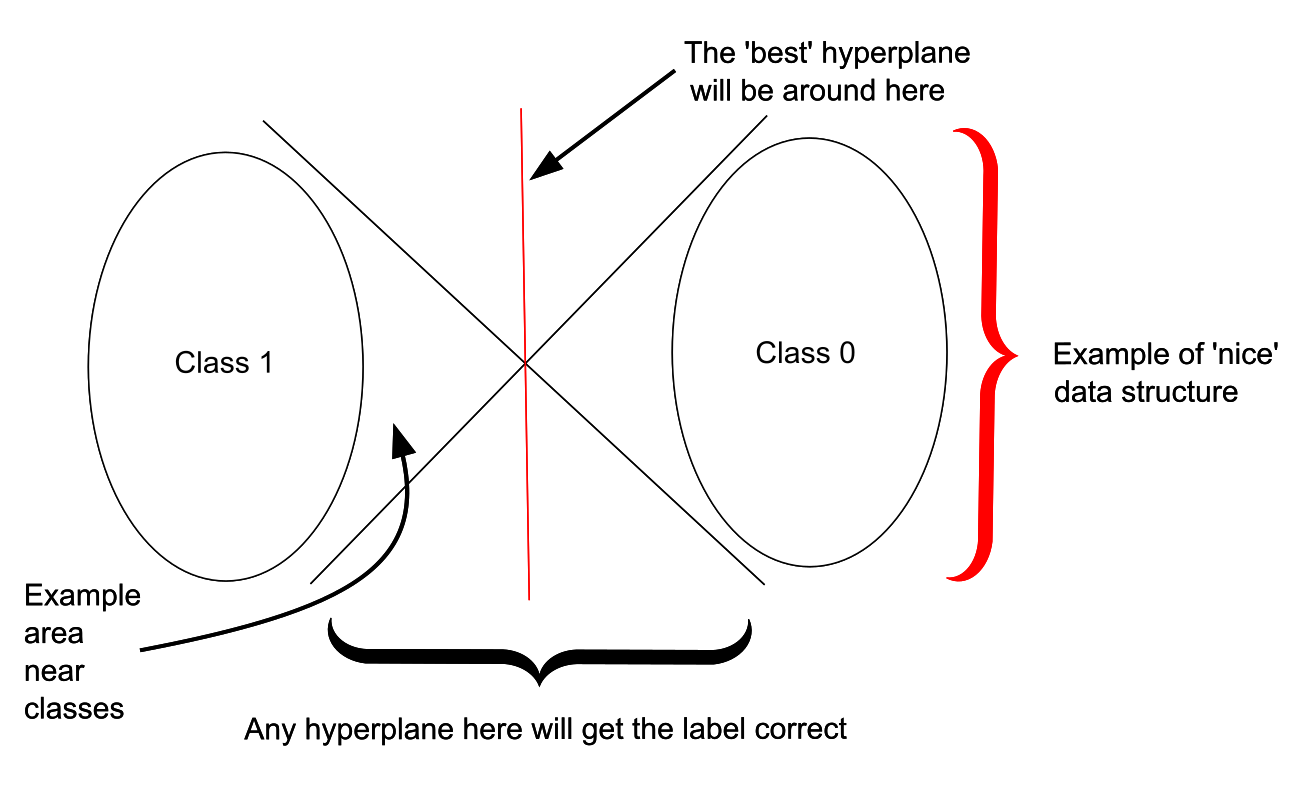
\includegraphics[width=\textwidth]{figs/hyperplanes_good_classes.png}
\caption{Illustration of well separated classes.} 
\label{fig:good_sep_classes} % labels must come after captions (figures are 'labelable'?)
\end{figure}

Figure \ref{fig:good_sep_classes} shows the desired geometry of the data. In the following two scenarios our reasoning makes the assumption when new examples are fed into the algorithm, they will likely be somewhere around the existing classes. The ovals indicate the \enquote{clouds} of data that define each class and each line indicates a \gls{decisionboundary}. In a 2D context, this is a line and in a n-d context, these would be \gls{hyperplane}s.  For illustrative purposes, this is a 2D scenario, but it is important to recognise this would generalise up to n-many dimensions.  %In this instance, 

\begin{figure}[H]
    \centering
    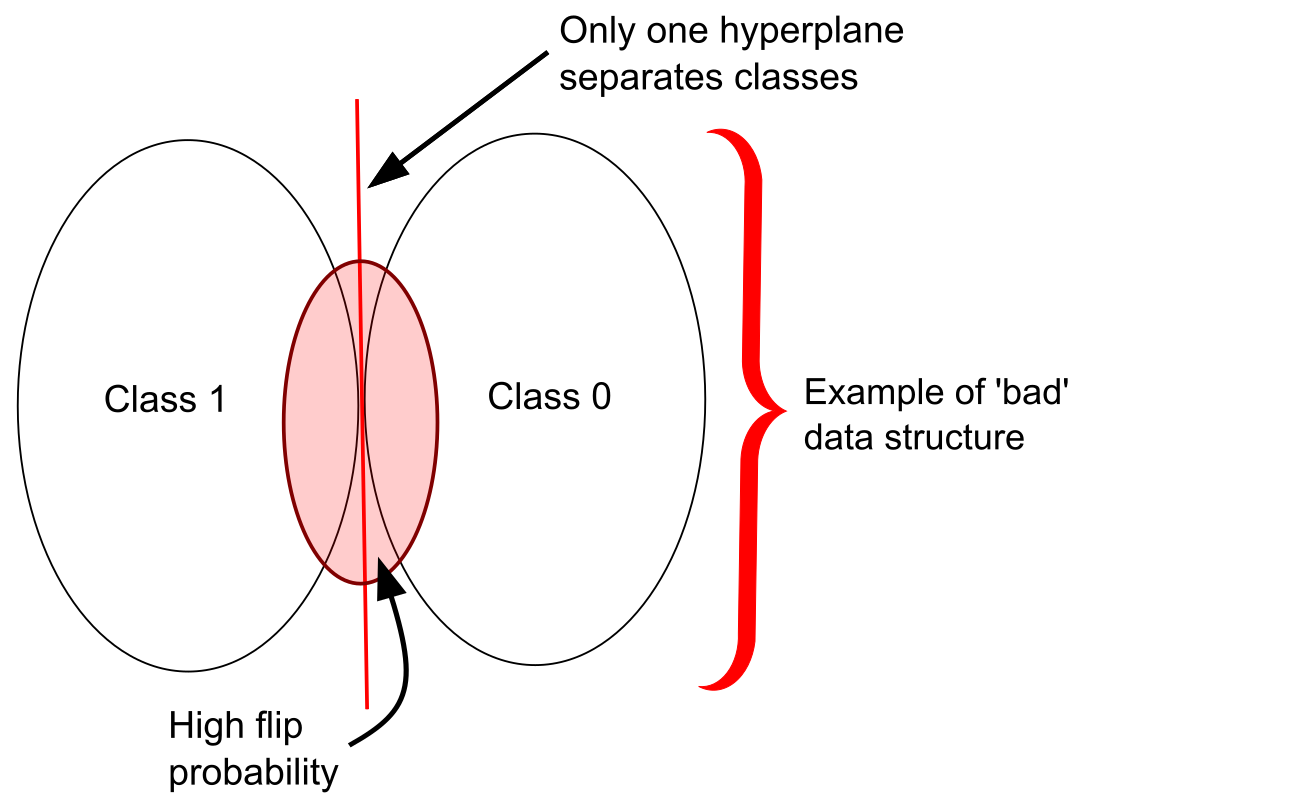
\includegraphics[width=\textwidth]{figs/hyperplanes_poor_classes.png}
    \caption[Illustration of poorly separated classes.]{With classes that have data grouped close together geometrically, we see there is a smaller range of separating hyperplanes that can be found (in this strictly hypothetically instance, there is only one meaningfully distinct hyperplane) and if we draw new samples from these classes, we might expect the data generating process to generate examples that are misclassified (and so experience a label \enquote{flip}) by the trained classifier.}
    \label{fig:poor_sep_classes}
\end{figure}

Figure \ref{fig:poor_sep_classes} shows a geometry of the data that would have high flipping probability upon \gls{rp}. There is only one \gls{hyperplane} that separates the classes. Hence new examples (e.g. out-of-sample data), which are likely to be near this boundary (the area indicated in red) have a high chance of being misclassified. This is an example of a situation where a traditional loss function, such as the \gls{mse}, would have poor \gls{generalisationperformance}, upon learning a \gls{decisionboundary} between these two classes. \bigskip

Calculation of empirical \gls{fp} (compressing the data via \gls{rp}s) allows for a proxy of how separable the classes are. However, any single \gls{rp} is not likely to find a good representation of the data. We define a \enquote{good representation} as a representation that allows for accurate and rapidly learning on the data, compared to attempting to learn on a \enquote{raw} untransformed version of the data.

% the above paragraph fails to mention the disconnect between gradient based learning and using flip probability - you need to mention this somewhere

Hence, we wish to find a good representation of the data, through many repeated  \gls{rp}s, that shifts the classes away from each other geometrically (i.e. from Figure \ref{fig:poor_sep_classes} to Figure \ref{fig:good_sep_classes}) and hence minimises the \gls{fp} \bigskip

For this, we will need an empirical measure of \gls{fp} and a functioning (trainable) implementation of it in a \gls{cnn}. \bigskip

\gls{fp}